% Created by tikzDevice version 0.10.1 on 2018-02-16 11:01:25
% !TEX encoding = UTF-8 Unicode
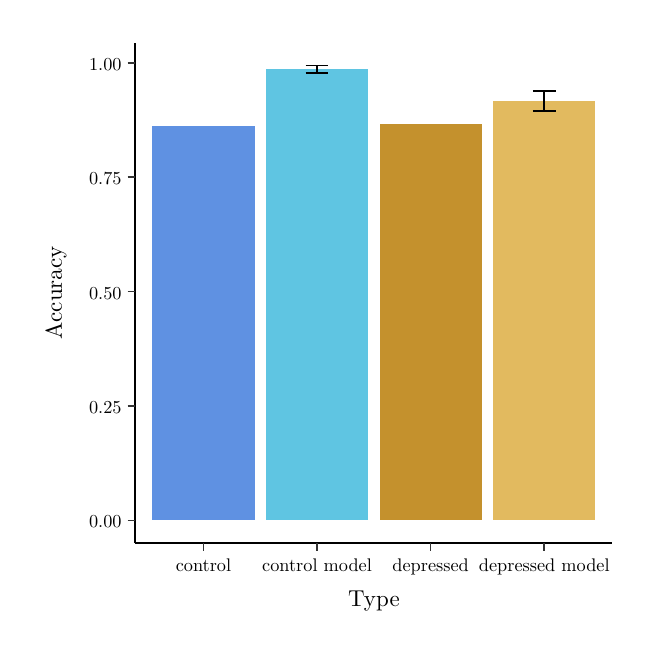
\begin{tikzpicture}[x=1pt,y=1pt]
\definecolor{fillColor}{RGB}{255,255,255}
\path[use as bounding box,fill=fillColor,fill opacity=0.00] (0,0) rectangle (216.81,216.81);
\begin{scope}
\path[clip] (  0.00,  0.00) rectangle (216.81,216.81);
\definecolor{drawColor}{RGB}{255,255,255}
\definecolor{fillColor}{RGB}{255,255,255}

\path[draw=drawColor,line width= 0.6pt,line join=round,line cap=round,fill=fillColor] (  0.00,  0.00) rectangle (216.81,216.81);
\end{scope}
\begin{scope}
\path[clip] ( 38.88, 30.56) rectangle (211.31,211.31);
\definecolor{fillColor}{RGB}{255,255,255}

\path[fill=fillColor] ( 38.88, 30.56) rectangle (211.31,211.31);
\definecolor{fillColor}{RGB}{95,145,226}

\path[fill=fillColor] ( 45.04, 38.77) rectangle ( 81.99,181.38);
\definecolor{fillColor}{RGB}{95,197,226}

\path[fill=fillColor] ( 86.10, 38.77) rectangle (123.04,201.71);
\definecolor{fillColor}{RGB}{196,145,45}

\path[fill=fillColor] (127.15, 38.77) rectangle (164.10,181.94);
\definecolor{fillColor}{RGB}{226,186,95}

\path[fill=fillColor] (168.20, 38.77) rectangle (205.15,190.25);
\definecolor{drawColor}{RGB}{0,0,0}

\path[draw=drawColor,line width= 0.6pt,line join=round] (100.46,203.09) --
	(108.68,203.09);

\path[draw=drawColor,line width= 0.6pt,line join=round] (104.57,203.09) --
	(104.57,200.32);

\path[draw=drawColor,line width= 0.6pt,line join=round] (100.46,200.32) --
	(108.68,200.32);

\path[draw=drawColor,line width= 0.6pt,line join=round] (182.57,193.91) --
	(190.78,193.91);

\path[draw=drawColor,line width= 0.6pt,line join=round] (186.68,193.91) --
	(186.68,186.60);

\path[draw=drawColor,line width= 0.6pt,line join=round] (182.57,186.60) --
	(190.78,186.60);
\end{scope}
\begin{scope}
\path[clip] (  0.00,  0.00) rectangle (216.81,216.81);
\definecolor{drawColor}{RGB}{0,0,0}

\path[draw=drawColor,line width= 0.6pt,line join=round] ( 38.88, 30.56) --
	( 38.88,211.31);
\end{scope}
\begin{scope}
\path[clip] (  0.00,  0.00) rectangle (216.81,216.81);
\definecolor{drawColor}{RGB}{0,0,0}

\node[text=drawColor,anchor=base east,inner sep=0pt, outer sep=0pt, scale=  0.66] at ( 33.93, 36.04) {0.00};

\node[text=drawColor,anchor=base east,inner sep=0pt, outer sep=0pt, scale=  0.66] at ( 33.93, 77.38) {0.25};

\node[text=drawColor,anchor=base east,inner sep=0pt, outer sep=0pt, scale=  0.66] at ( 33.93,118.72) {0.50};

\node[text=drawColor,anchor=base east,inner sep=0pt, outer sep=0pt, scale=  0.66] at ( 33.93,160.06) {0.75};

\node[text=drawColor,anchor=base east,inner sep=0pt, outer sep=0pt, scale=  0.66] at ( 33.93,201.39) {1.00};
\end{scope}
\begin{scope}
\path[clip] (  0.00,  0.00) rectangle (216.81,216.81);
\definecolor{drawColor}{gray}{0.20}

\path[draw=drawColor,line width= 0.6pt,line join=round] ( 36.13, 38.77) --
	( 38.88, 38.77);

\path[draw=drawColor,line width= 0.6pt,line join=round] ( 36.13, 80.11) --
	( 38.88, 80.11);

\path[draw=drawColor,line width= 0.6pt,line join=round] ( 36.13,121.45) --
	( 38.88,121.45);

\path[draw=drawColor,line width= 0.6pt,line join=round] ( 36.13,162.78) --
	( 38.88,162.78);

\path[draw=drawColor,line width= 0.6pt,line join=round] ( 36.13,204.12) --
	( 38.88,204.12);
\end{scope}
\begin{scope}
\path[clip] (  0.00,  0.00) rectangle (216.81,216.81);
\definecolor{drawColor}{RGB}{0,0,0}

\path[draw=drawColor,line width= 0.6pt,line join=round] ( 38.88, 30.56) --
	(211.31, 30.56);
\end{scope}
\begin{scope}
\path[clip] (  0.00,  0.00) rectangle (216.81,216.81);
\definecolor{drawColor}{gray}{0.20}

\path[draw=drawColor,line width= 0.6pt,line join=round] ( 63.52, 27.81) --
	( 63.52, 30.56);

\path[draw=drawColor,line width= 0.6pt,line join=round] (104.57, 27.81) --
	(104.57, 30.56);

\path[draw=drawColor,line width= 0.6pt,line join=round] (145.62, 27.81) --
	(145.62, 30.56);

\path[draw=drawColor,line width= 0.6pt,line join=round] (186.68, 27.81) --
	(186.68, 30.56);
\end{scope}
\begin{scope}
\path[clip] (  0.00,  0.00) rectangle (216.81,216.81);
\definecolor{drawColor}{RGB}{0,0,0}

\node[text=drawColor,anchor=base,inner sep=0pt, outer sep=0pt, scale=  0.66] at ( 63.52, 20.15) {control};

\node[text=drawColor,anchor=base,inner sep=0pt, outer sep=0pt, scale=  0.66] at (104.57, 20.15) {control model};

\node[text=drawColor,anchor=base,inner sep=0pt, outer sep=0pt, scale=  0.66] at (145.62, 20.15) {depressed};

\node[text=drawColor,anchor=base,inner sep=0pt, outer sep=0pt, scale=  0.66] at (186.68, 20.15) {depressed model};
\end{scope}
\begin{scope}
\path[clip] (  0.00,  0.00) rectangle (216.81,216.81);
\definecolor{drawColor}{RGB}{0,0,0}

\node[text=drawColor,anchor=base,inner sep=0pt, outer sep=0pt, scale=  0.83] at (125.10,  7.83) {Type};
\end{scope}
\begin{scope}
\path[clip] (  0.00,  0.00) rectangle (216.81,216.81);
\definecolor{drawColor}{RGB}{0,0,0}

\node[text=drawColor,rotate= 90.00,anchor=base,inner sep=0pt, outer sep=0pt, scale=  0.83] at ( 12.32,120.93) {Accuracy};
\end{scope}
\end{tikzpicture}
